% turbo-sc10.tex

\section{Subsonic compressor blade -- sc10}
%
Standard-condition 10 for a two-dimensional compressor blade with subsonic flow.
The main objective is to provide a solution of a transonic flow for comparison with 
the solution produced by Paul Petrie-Repar's RPMTurbo code.
The geometry for this example was set up in \texttt{mbcns2} by Hannes Wojciak and Paul Petrie-Repar.
The UDF boundary conditions for a periodic boundary were later completed by PJ.
%

\begin{figure}[htbp]
\begin{center}

\includegraphics[width=12cm, viewport=0 0 456 326]{../2D/turbo_sc10/sc10-edited.pdf}
\end{center}
\caption{Overview of the flow geometry, showing the interior block boundaries 
  and a number of anchor points.
  A number of the automatically-generated labels have been removed and
  others have been moved to make the diagram clearer.}
\label{trubo-sc10-overall-geometry-fig}
\end{figure}

\begin{figure}[htbp]
\begin{center}

\includegraphics[width=12cm,viewport=132 44 313 280,clip]{../2D/turbo_sc10/sc10-inner.pdf}
\end{center}
\caption{A further-edited diagram showing the blade surface and the arrangement
  of the inner blocks.  More of the anchor-points are labelled. }
\label{trubo-sc10-inner-geometry-fig}
\end{figure}

\begin{figure}[htbp]
\begin{center}
\includegraphics[width=0.9\textwidth,viewport=24 495 570 817]{../2D/turbo_sc10/mesh.pdf}
\end{center}
\caption{Mesh around the subsonic compressor blade.}
\label{turbo-sc10-meshfig}
\end{figure}

\begin{figure}[htbp]
\begin{center}
\includegraphics[width=0.9\textwidth,viewport=24 495 570 817]{../2D/turbo_sc10/mach-field.pdf}
\end{center}
\caption{Mach number field for flow over a subsonic compressor blade.}
\label{turbo-sc10-mach-fig}
\end{figure}

\begin{figure}[htbp]
\begin{center}
\includegraphics[width=0.9\textwidth,viewport=24 495 570 817]{../2D/turbo_sc10/pressure-field.pdf}
\end{center}
\caption{Pressure field for flow over a subsonic compressor blade.}
\label{turbo-sc10-pressure-fig}
\end{figure}


\begin{figure}[htbp]
\begin{center}
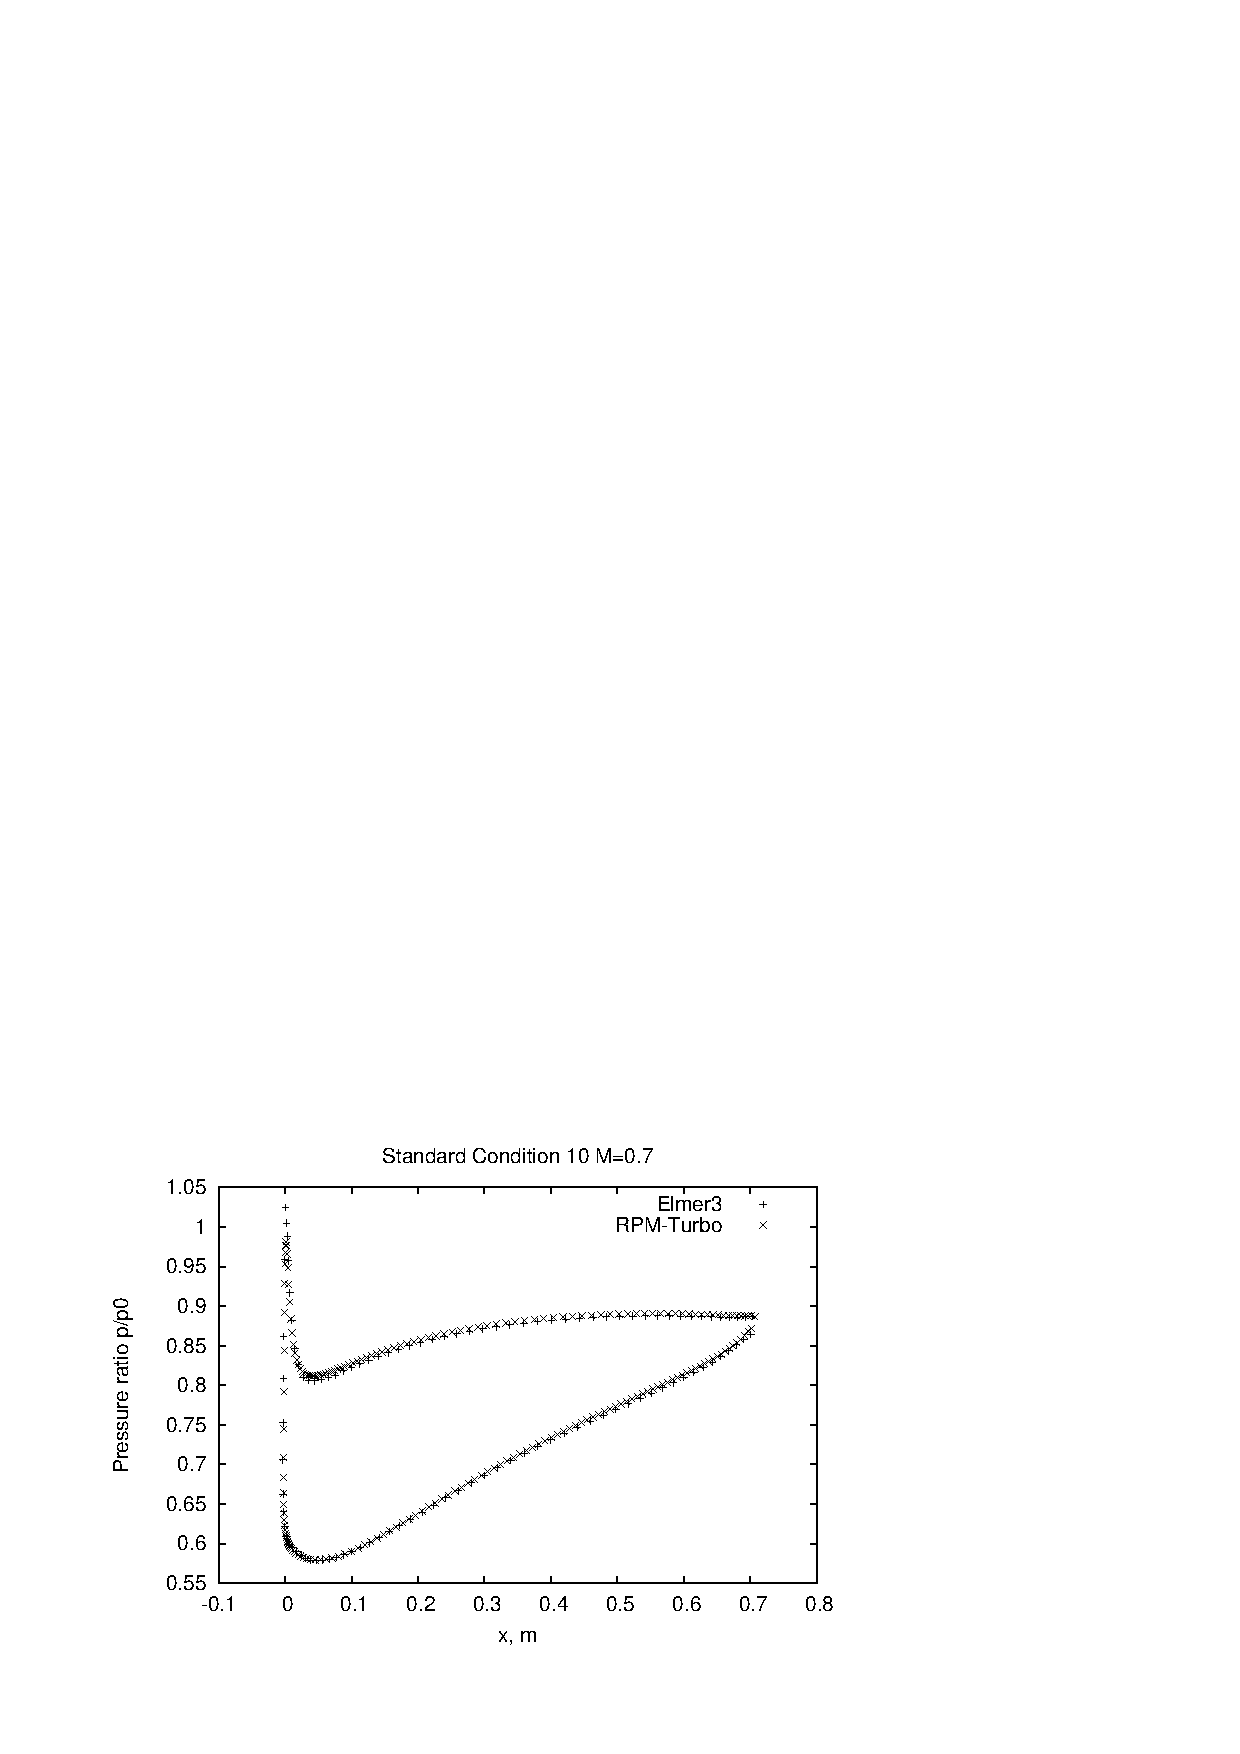
\includegraphics[width=10cm]{../2D/turbo_sc10_parametric/surface_p.pdf}
\end{center}
\caption{Pressure around the blade surface; comparison with RPM-Turbo reference data.}
\label{turbo-sc10-surface-p-fig}
\end{figure}


\subsection{Input script (.py)}
\topbar
\lstinputlisting[language={}]{../2D/turbo_sc10/sc10.py}
\bottombar


\subsection{Boundary-condition files (.lua)}
\topbar
\lstinputlisting[language={}]{../2D/turbo_sc10/udf-subsonic-sc10.lua}
\bottombar \\
\topbar
\lstinputlisting[language={}]{../2D/turbo_sc10/udf-periodic-bc.lua}
\bottombar


\subsection{Shell scripts}
\label{turbo-sc10-sh-files}
\topbar
\lstinputlisting[language={}]{../2D/turbo_sc10/sc10_prep.sh}
\bottombar \\
\topbar
\lstinputlisting[language={}]{../2D/turbo_sc10/sc10_run.sh}
\bottombar \\
\topbar
\lstinputlisting[language={}]{../2D/turbo_sc10/sc10_post.sh}
\bottombar

\subsection{Notes}
\begin{itemize}
\item Run time is approximately 11600 seconds for 276720 steps on a computer with 
      an AMD Phenom 9650 2.7\,GHz processor.
\end{itemize}
